\chapter{Theoretical Background and Market Analysis}
\label{chap:ch1}

This chapter establishes the foundational context necessary to understand the architectural and functional decisions made throughout the development of the proposed scheduling application. Bridging the gap between the operational challenges identified in the previous chapter and the technical implementations detailed in subsequent sections, this chapter is divided into two primary domains: theoretical frameworks and market analysis.

First, the theoretical background explores the academic and computational principles that underpin modern workforce management systems. It examines the computational complexities of utilizing \textbf{Constraint Satisfaction Problems (CSP)} \cite{csp_processing} for algorithmic scheduling, the structural paradigms required to build secure, Multi-Tenant Software-as-a-Service (SaaS) architectures and the importance of Context-Aware Data Isolation. \cite{ContextAwareDataIsolation}

Following this theoretical grounding, a comprehensive market analysis is presented. By evaluating the current global software landscape and analyzing the capabilities of leading commercial solutions, this section identifies critical functional and architectural gaps - particularly for small-to-medium enterprises requiring highly localized business logic. This dual approach, combining academic theory with pragmatic industry realities, serves to justify the system's design choices and highlights the project's unique value proposition within the broader digital economy.

\begin{table}[H]
\centering
\caption{Context Summary}
\label{tab:chapter_context}
\renewcommand{\arraystretch}{0.8}
\begin{tabular}{|p{4.5cm}|p{11cm}|}
\hline
\textbf{Area} & \textbf{Key Idea} \\ \hline
Theory & CSP-based scheduling, SaaS multi-tenancy, and Context-Aware Data Isolation for scalable workforce systems. \\ \hline
Market & Analysis of existing tools highlighting gaps in flexibility, scalability, and SME/local business suitability. \\ \hline
\end{tabular}
\end{table}


\begin{figure}[!h]
    \centering
    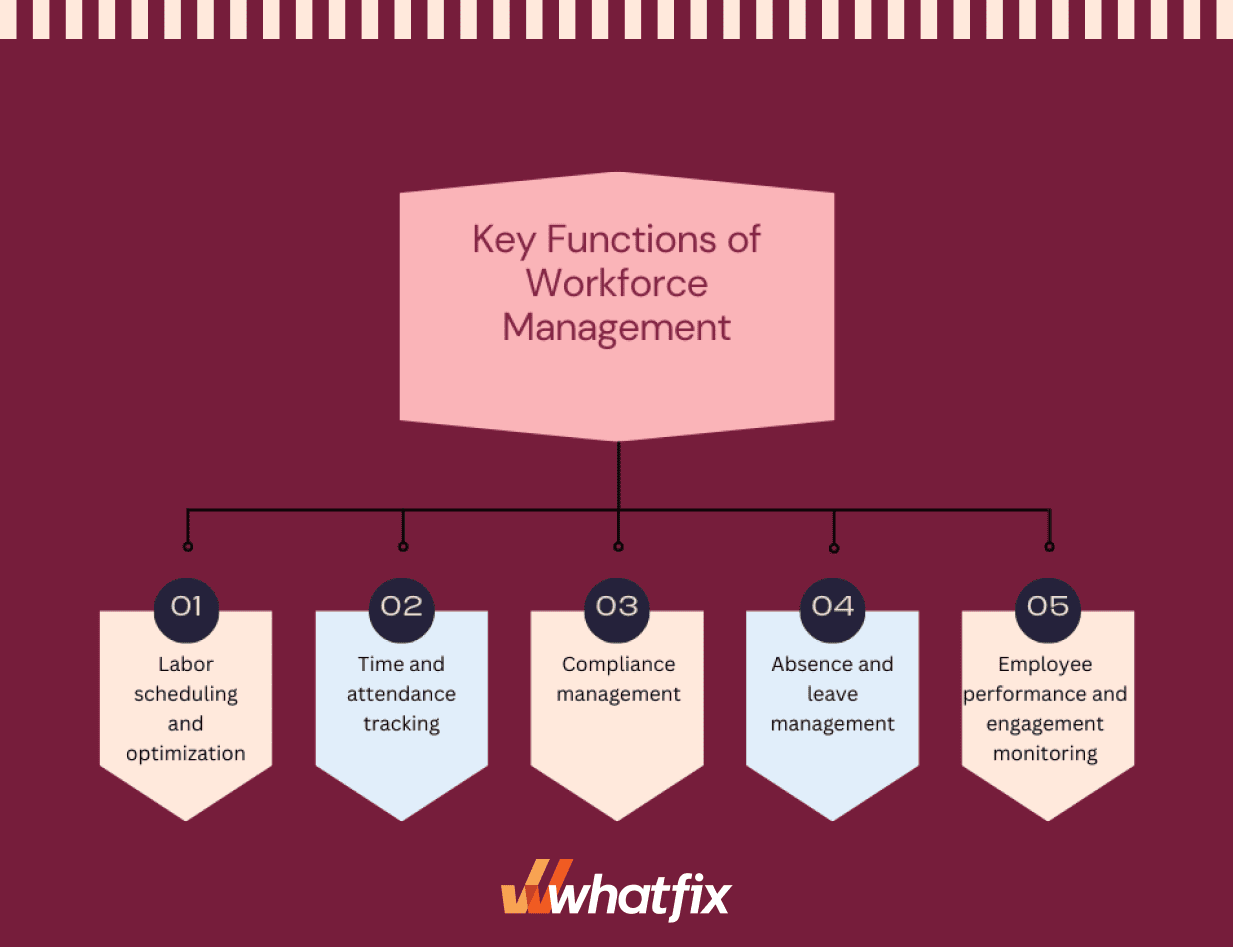
\includegraphics[width=1\linewidth]{Workforce.png}
    \caption{Overview of workforce management features}
    \label{fig:workflowFeatures}
\end{figure}.

\section{Theoretical Frameworks in Software Architecture}
\subsection{Constraint Satisfaction Problems in Automated Scheduling}

The foundation of modern algorithmic scheduling lies in the field of artificial intelligence and operations research, specifically within the domain of Constraint Satisfaction Problems (CSP). A CSP is defined mathematically by a set of variables (e.g., available work shifts), a domain of values for each variable (e.g., the pool of available employees), and a set of constraints that restrict the allowable combinations of values. \cite{Meseguer1989}

In workforce management, these constraints are categorized as either hard or soft. Hard constraints are non-negotiable boundaries, such as legal maximum weekly working hours or mandatory rest periods between shifts. Soft constraints represent operational preferences, such as an employee's desire to work morning shifts or a manager's preference to balance out the working hours for each employee. The theoretical challenge—and computational complexity—of automated scheduling systems lies in designing algorithms capable of navigating these multi-dimensional constraints to find an optimal, legally compliant assignment without requiring exponential computational time.

\subsection{Multi-Tenant Software-as-a-Service (SaaS) Paradigms}
 
The architectural shift from locally hosted, single-tenant applications to a future cloud-based Software-as-a-Service (SaaS) platforms requires robust Multi-Tenancy models. Multi-tenancy refers to a software architecture in which a single instance of an application serves multiple distinct user groups, or "tenants."\cite{MultiTenantSaaS}

From a theoretical standpoint, multi-tenant data architecture generally falls into three categories: isolated databases, isolated schemas within a shared database, or a shared database with shared schemas. Modern SaaS platforms frequently employ the latter for its scalability and cost-efficiency. However, this approach necessitates strict programmatic barriers—often termed Context-Aware Data Isolation—to ensure that a tenant (e.g., an independent store branch) cannot access or manipulate the data of another tenant, requiring security logic to be deeply embedded into the application's data persistence layer.

\begin{figure}[!h]
    \centering
    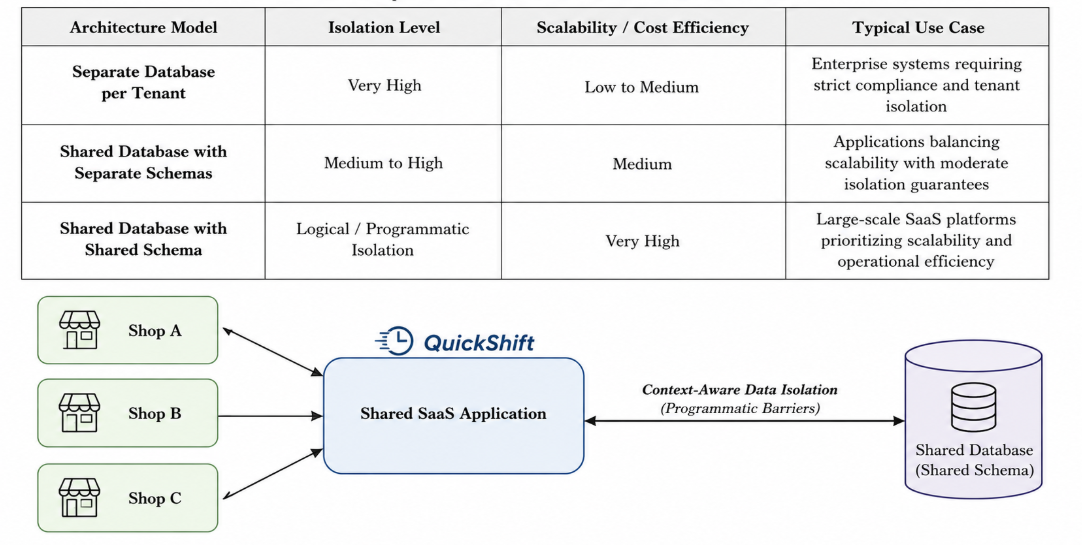
\includegraphics[width=1\linewidth]{SharedSchema.png}
    \caption{Shared Database Schema and table}
    \label{fig:placeholder}
\end{figure}

\subsection{Advanced Role-Based Access Control (RBAC) and Stateless Authentication}

To support secure multi-tenancy, access control mechanisms have evolved significantly. Traditional, stateful session-based authentication has largely been superseded by stateless protocols utilizing JSON Web Tokens (JWT).

While basic Role-Based Access Control (RBAC) relies on checking a user's assigned role against a requested endpoint (e.g., validating if a user has "ADMIN" privileges), enterprise-grade systems require Layer 2 Data-Level RBAC. In this theoretical model, access control is not merely a gatekeeper at the application's edge; rather, the authentication identity is injected directly into the data querying process. This ensures that data retrieval is dynamically scoped to the user's specific organizational context, rendering unauthorized horizontal data access architecturally impossible.\cite{RBAC1}

\section{Market Analysis of Workforce Management Solutions}
\subsection{Global Market Dynamics and Growth Indicators}

The demand for intelligent workforce management solutions is experiencing rapid and sustained growth, driven by increasing emphasis on operational efficiency and labor compliance. According to recent industry projections, the global Employee Scheduling and Shift Planning Software market is expected to grow from approximately USD 1.89 billion in 2024 to nearly USD 3.94 billion by 2032, representing a Compound Annual Growth Rate (CAGR) of 9.6\%. \cite{SchedulingMarket2024}.\begin{equation}
\text{CAGR} = \left( \frac{V_{final}}{V_{begin}} \right)^{\frac{1}{t}} - 1
\end{equation}
This expansion is largely fueled by the transition of Small and Medium Enterprises (SMEs) away from manual spreadsheet-based scheduling toward centralized, cloud-based Software-as-a-Service (SaaS) platforms that provide automated workforce optimization and compliance management.

\begin{figure}[H]
    \centering
    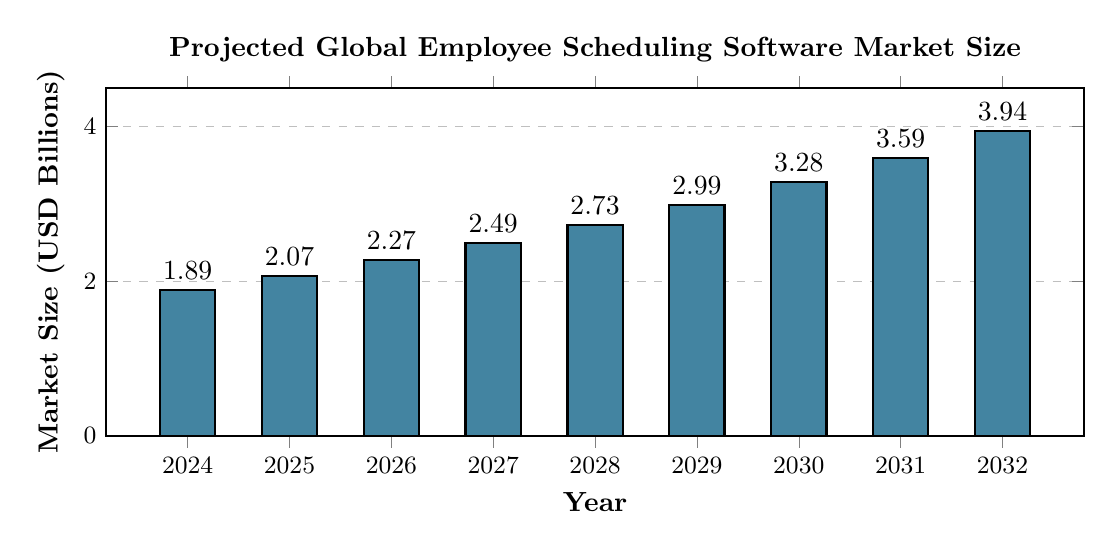
\begin{tikzpicture}
        \begin{axis}[
            ybar,
            bar width=20pt,
            width=14cm,
            height=6cm,
            title={\textbf{Projected Global Employee Scheduling Software Market Size}},
            xlabel={Year},
            ylabel={Market Size (USD Billions)},
            symbolic x coords={2024, 2025, 2026, 2027, 2028, 2029, 2030, 2031, 2032},
            xtick=data,
            nodes near coords, % Displays the values on top of the bars
            nodes near coords align={vertical},
            ymin=0, ymax=4.5,
            enlarge x limits=0.1,
            % Styling the chart for a professional thesis look
            axis line style={thick},
            tick label style={font=\small},
            label style={font=\normalsize\bfseries},
            ymajorgrids=true,
            grid style=dashed,
        ]
            % Data calculated using: 1.89 * (1 + 0.096)^(Year - 2024)
            \addplot[fill=cyan!60!black, draw=black, thick] coordinates {
                (2024, 1.89)
                (2025, 2.07)
                (2026, 2.27)
                (2027, 2.49)
                (2028, 2.73)
                (2029, 2.99)
                (2030, 3.28)
                (2031, 3.59)
                (2032, 3.94)
            };
        \end{axis}
    \end{tikzpicture}
    \caption{Projected market growth from 2024 to 2032.}
    \label{fig:market_growth_projection}
\end{figure}

\subsection{Ecosystem of Leading Competitors}

The current commercial landscape is dominated by several large-scale SaaS providers, each targeting broad demographics of shift-based industries:

\begin{itemize}
    \item \textbf{Deputy:} Recognized as a market leader, Deputy provides a comprehensive suite of workforce management tools. Its core strengths lie in automated scheduling based on robust historical data and extensive integrations with third-party payroll systems. It is primarily built for medium-to-large enterprises in retail and hospitality \cite{Deputy}.
    
    \item \textbf{ShiftIn:} Targeted at small and medium Romanian businesses, ShiftIn offers closer maintenance support with more customization for a monthly, subscription fee. \cite{ShiftIn}.

    \item \textbf {Homebase:} Targeted more aggressively at small businesses, Homebase offers an accessible entry point with core features like drag-and-drop scheduling, basic team communication, and time-tracking. \cite{Homebase}
    
    \item \textbf{When I Work:} This platform differentiates itself through strong mobile-first employee self-service capabilities, allowing workers to easily trade shifts, request time off, and manage their availability directly from their smartphones. \cite{WhenIWork}

    
\end{itemize}

\subsection{Identifying the Architectural and Functional Gap}

Despite the maturity of the previously mentioned platforms, a critical analysis reveals significant structural gaps, particularly regarding niche adaptability and proactive automation for SMEs.

First, leading platforms operate on a "One-Size-Fits-All" paradigm. To accommodate every possible industry—from healthcare to construction. Their core employee models are overly generalized. Businesses requiring highly specific, localized HR metrics (such as unique holiday recovery tracking or strict contract-type delineations like "Part-Time 4H vs. 6H") often find these tools either incapable of enforcing these rules or requiring prohibitively expensive "Enterprise" tier customizations.

Furthermore, while current systems excel at reactive scheduling—such as allowing an employee to drop a shift and notifying a manager to manually find a replacement—there is a distinct lack of proactive algorithmic automation. Existing platforms either rely on manual managerial intervention to resolve last-minute staffing shortages, or assign the shift just to the first eligible worker.s QuickShift addresses this limitation through its \texttt{findBestCandidate} function, which automatically evaluates labor constraints and individual preferences to identify and assign the optimal replacement worker, rather than merely the first available one. 

\begin{figure}[!h]
    \centering
    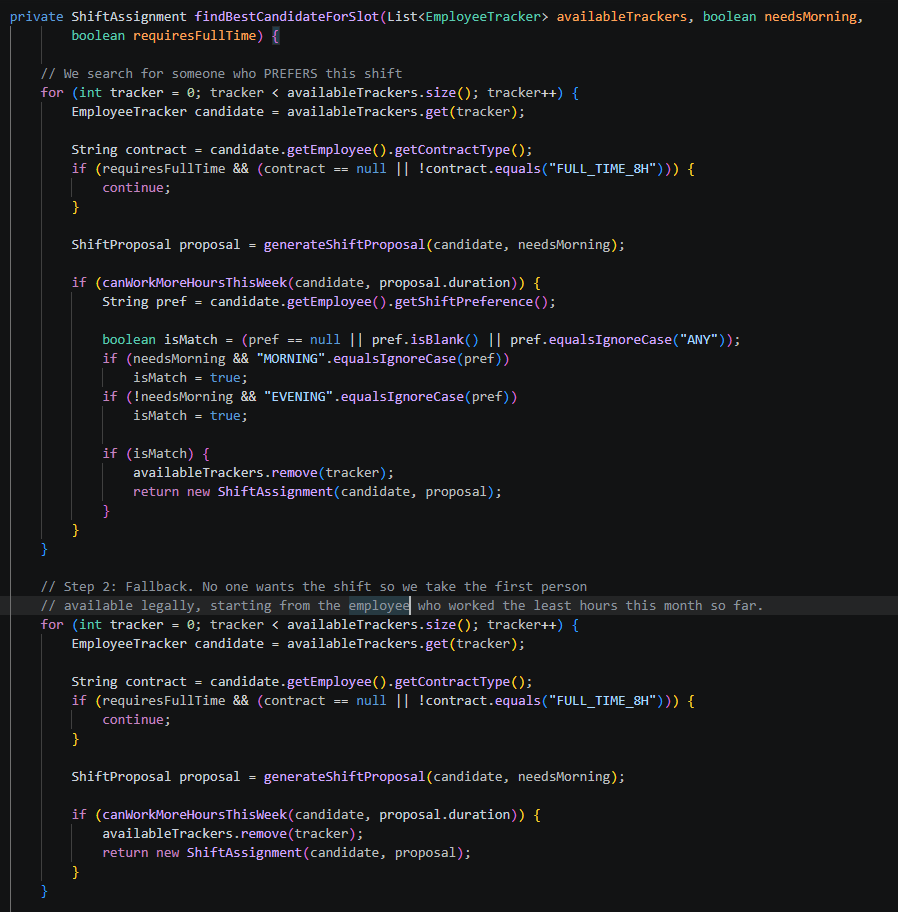
\includegraphics[width=0.7\linewidth]{findBestCandidate.png}
    \caption{findBestCandidate function}
    \label{fig:placeholder}
\end{figure}

This identified gap between generalized, reactive software and the need for highly specific, automated operational continuity forms the foundational premise for the architectural solutions proposed in the subsequent chapters.